\subsection{Trigger system}

During LHC Run 2, and at the start of Run 3, the LHC provides collisions to CMS at a rate of 40 MHz due to the spacing between bunches of protons. It is not feasible for the CMS detector to save recorded information from all collisions, as the on-detector electronics buffers would fill and halt the incoming flow of data. Additionally, this would lead to a very large amount of required offline storage space. 

In order to reduce the rate of data saved by the detector, CMS employs a two tiered trigger system in order to pre-select interesting physics events at the hardware level.. The first level, the Level 1 (L1) trigger, reduces the rate of data stored to 100 kHz. The second level, the High Level Trigger (HLT) further reduces this rate to 1 kHz. 

\subsubsection{Level 1 Trigger}

The CMS L1 trigger makes an initial judgement on the incoming data in order to determine if a physics event is worth keeping or not. The inputs into the CMS L1 are Trigger Primitives (TP) formed by individual subsystems, and the output is a decision on whether or not to save data for further processing. A diagram of the CMS Level-1 trigger is shown in Figure \ref{fig:CMS_L1_Trigger} \cite{Sirunyan_2020}.

\begin{figure}[H]
    \centering
    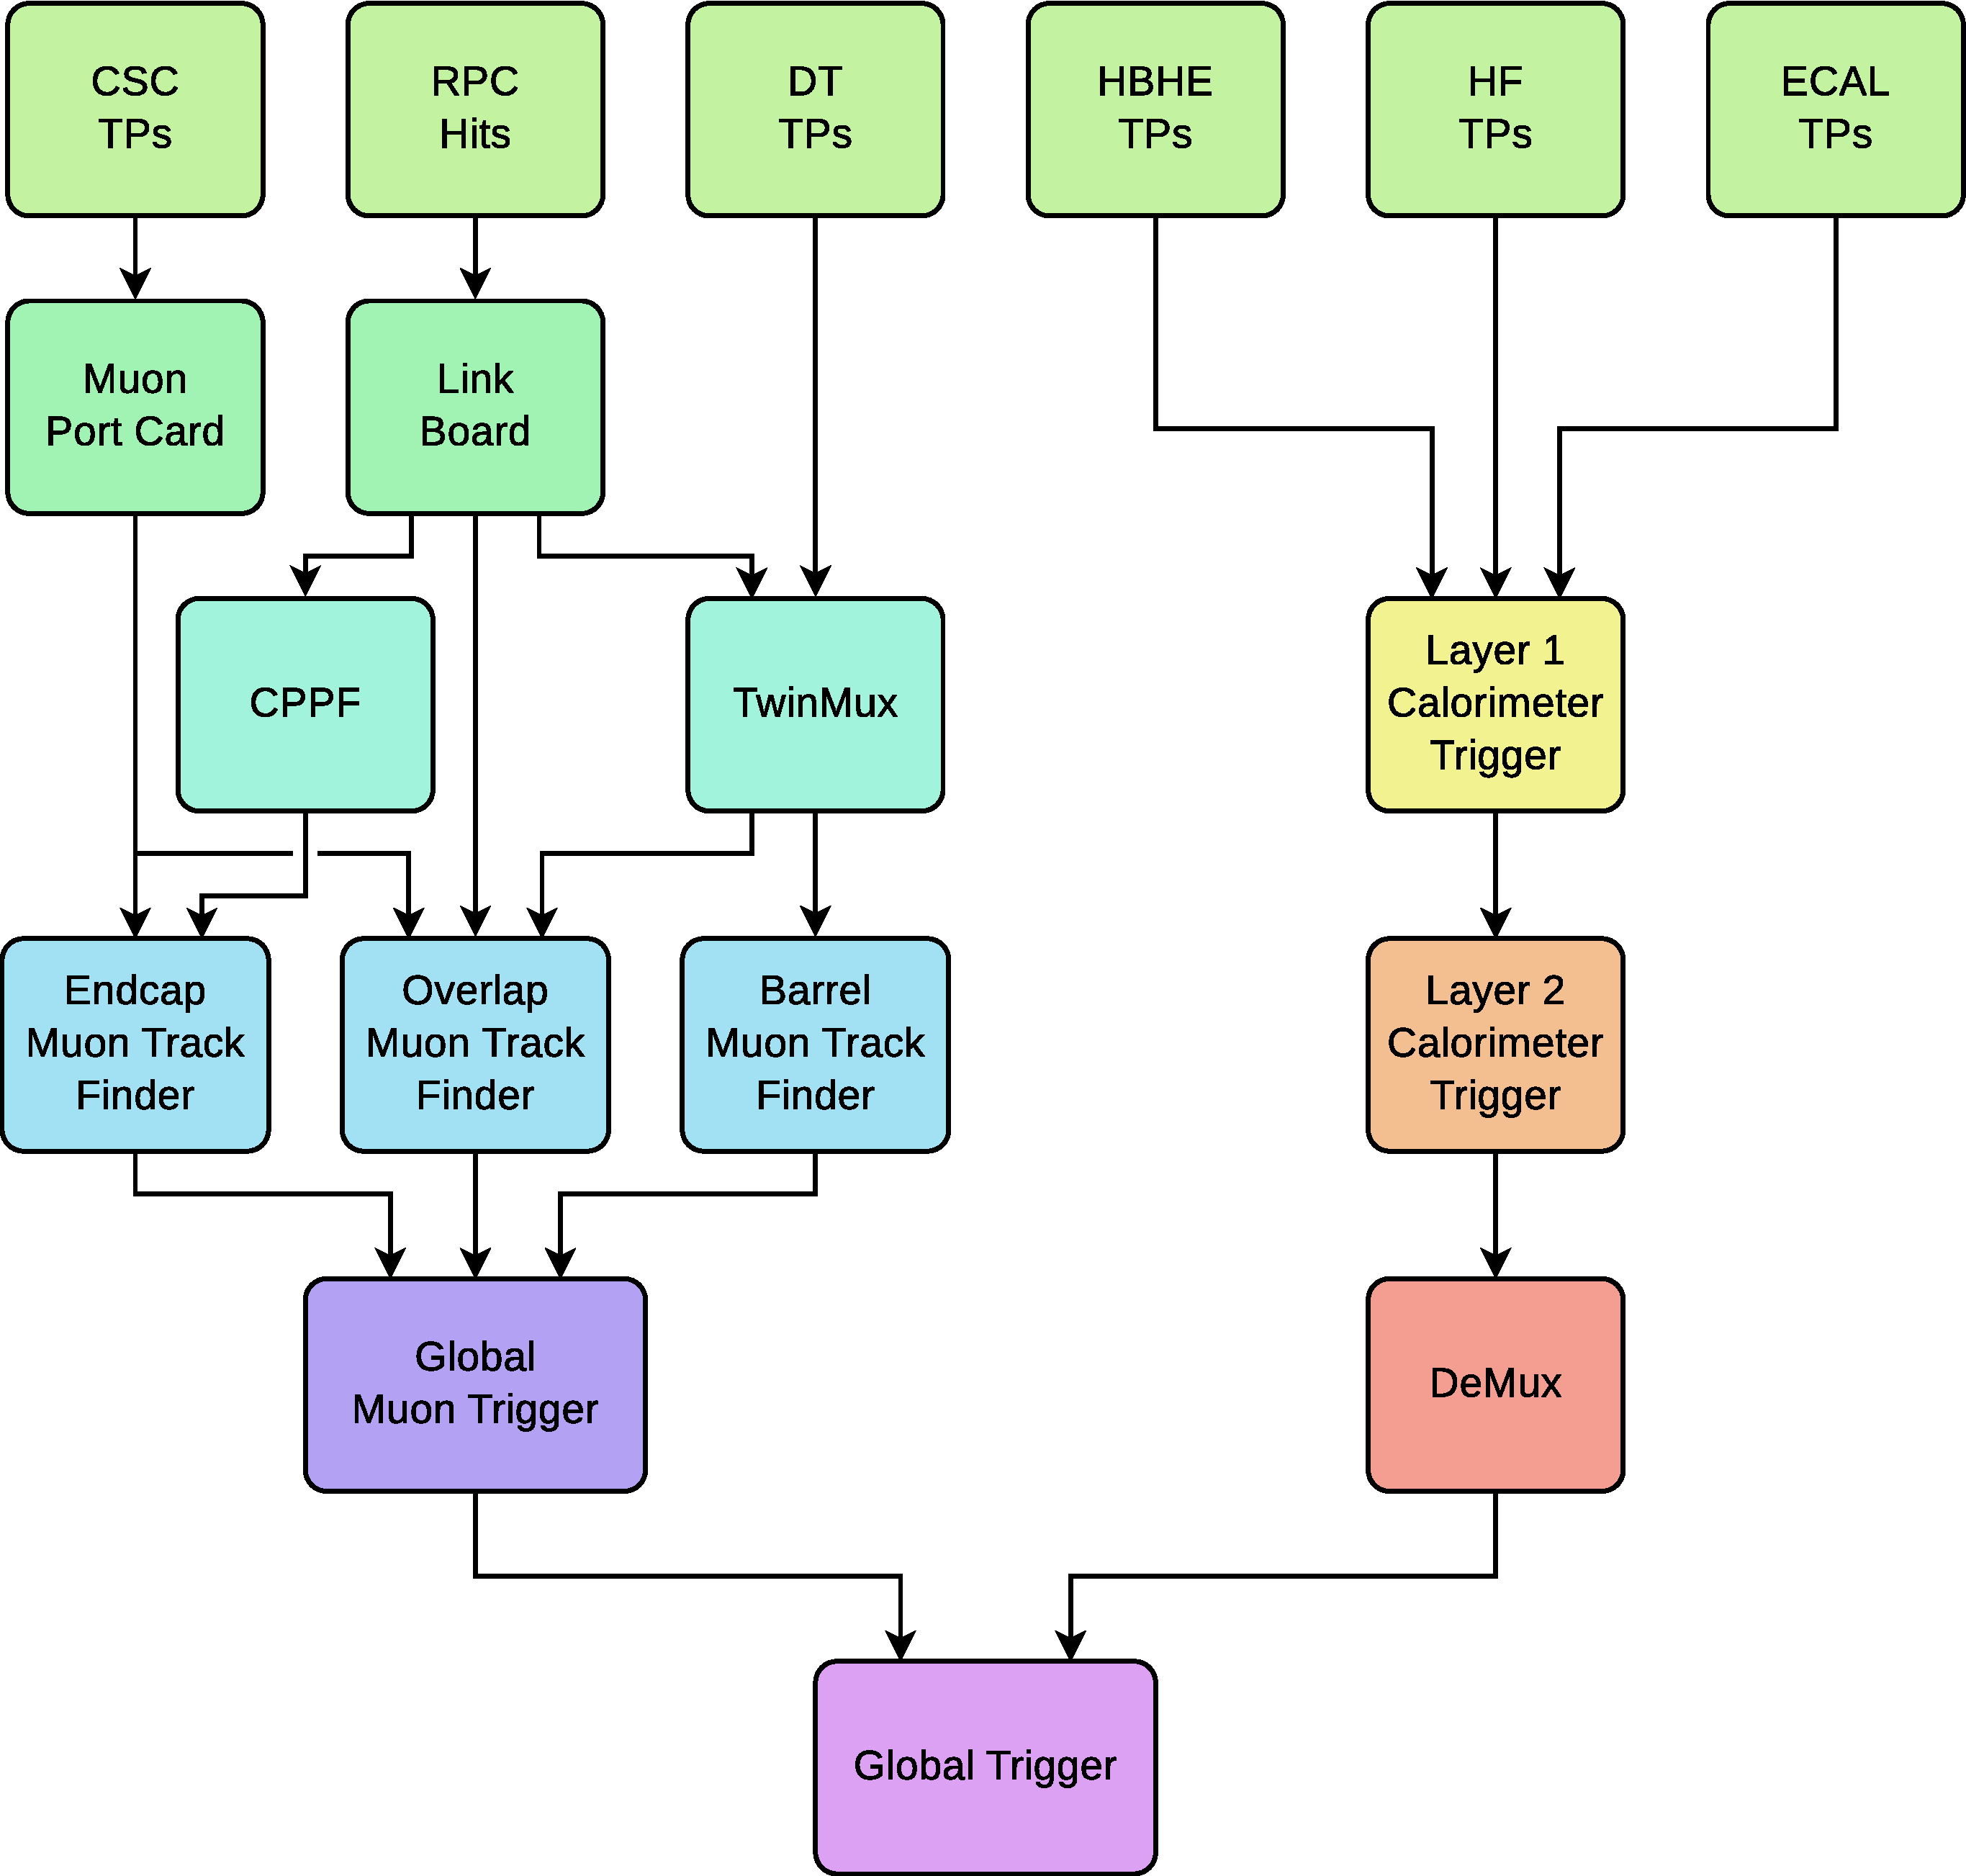
\includegraphics[width=0.75\textwidth]{Images/Trigger/CMS_L1_Trigger.pdf}
    \caption{The CMS Level-1 Trigger}
    \label{fig:CMS_L1_Trigger}
\end{figure}

It is imperative that Level-1 decisions are made in a timely fashion, quickly enough such that the on-detector electronics buffers do not fill. If this were to occur, the flow of incoming data would be halted and CMS would begin to lose events. It is for this reason that a latency of $\approx$4 $\mu$s is imposed as the maximum time limit for L1 to make a decision on whether or not to further process data from a bunch crossing (BX). 

During this $\approx$4 $\mu$s, TPs from the muon systems are input to the muon L1 algorithms: The EMTF (Endcap muon track finder), OMTF (Overlap muon track finder) and BMTF (Barrel muon track finder). These respective track finding algorithms make use of the multiple CMS muon sub-system information, and their outputs are all input to the Global Muon Trigger in order to build L1 muon objects. At the same time, the ECAL and HCAL TPs are input to the calorimeter layers: Calorimeter layers 1 and 2, which are responsible for producing L1 objects of the remaining physics objects of interest: EGamma (Electron or photon), jet, and tau objects. 

For a given event, this will result in a set of L1 objects. To determine whether or not an event passes the L1 trigger through a Level-1 accept (L1A), it is checked whether at least one of the Level-1 menu seeds meets the requirements of the event's L1 objects. If this is the case, an L1A is sent to the CMS sub-detectors in order to notify them to send the TP information stored in their on-detector electronics buffers to the central DAQ (Data acquisition) system for further processing at the HLT. It is for this reason that an appropriate level-1 menu must be designed based on the expected collisions delivered to CMS, and physics program the detector would like to pursue. 

During Run 2 and at the start of Run 3, the goal of the L1 trigger was to reduced the data-taking rate from 40 MHz to 100 kHz. 

A major update to the L1 trigger for CMS envisioned to be implemented for the Phase-II CMS detector, which will operate during the HL-LHC, is the addition of tracker information for making L1 decisions. This has the potentially to make L1 decisions based on a variety of additional physics signatures, including based on displayed vertices from b-quarks, potentially leading to much purer CMS datasets. 

\subsubsection{High Level Trigger}

% https://cms.cern/news/first-collisions-reconstructed-gpus-cms
% http://cds.cern.ch/record/2759072/files/CMS-TDR-022.pdf?version=3

After the L1 trigger makes an initial decision on which events recorded by CMS are interesting and warrant further inspection, reducing the data-taking rate from a maximum of 40 MHz to 100 kHz, events are passed to the HLT (High level trigger) to make a final decision on whether or not an event is saved at CMS. The HLT is a computing farm located above the CMS control room, which performs a reconstruction similar to the standard offline CMS event reconstruction on events passing the L1 trigger, and during Run 2 reduced the trigger rate from 100 kHz to 1 kHz for permanent storage. An image of the HLT computing farm is shown in Figure \ref{fig:HLT_Farm}.

\begin{figure}[H]
    \centering
    \includegraphics[width=0.7\textwidth]{Images/CMS/CMS_HLT_Farm.jpg}
    \caption{CMS HLT computing farm (2010)} % From 2010 
    \label{fig:HLT_Farm} % https://www.flickr.com/photos/irmp/4583961234
\end{figure}

During LS2, the CMS HLT began implementing the use of Graphical Processing Units (GPUs) in conjunction with CPUs (Central processing units) in order to decrease the time required to reconstruct physics events. The potential gain could be very useful for CMS, as if HLT processing time is decreased one would have more ``time budget'' to allocate to reconstruction, potentially allowing for more complex reconstruction, and to that end a purer dataset saved by the HLT farm. The CMS HLT is currently running with a combination of CPUs and GPUs, and has successfully commissioned this version of reconstruction for the start of LHC Run 3. 